\documentclass[twocolumn]{revtex4}
%\documentclass[onecolumn,12pt]{revtex4}
%\usepackage{amsfonts,amssymb,amsmath,mathbbol}              % for math symbols.
%\usepackage{epstopdf}
%\usepackage{mathbbol}              % for math symbols.
\usepackage{graphics,graphicx,epsfig,ulem} 
\usepackage{amsmath}

\begin{document}

\textheight=24.75cm

\title{Measuring the Heat Capacity of Air} 
 
 
\author{Jacky Cao, Lab Group A, Thursday,}


\begin{abstract}              
 
 
The maximum rise in pressure, $\Delta p$, for a given heating time, $\Delta T$, was measured by using a pressure meter connected to the glass bottle in the experiment. The final result for C\textsubscript{V} obtained from the data was 36.1$\pm0.6$Jmol\textsuperscript{-1}K\textsuperscript{-1}. This result is much larger than the expect result of C\textsubscript{V} = $\frac{5}{2}$R. The likely origin of this discrepancy could be due to the fact that pressure inside the bottle did not remain constant after the current was switched off, or possibly due to the fact that ambient infrared radiation would have been being absorbed by various parts of the apparatus. 

\end{abstract}

\maketitle

\section{Graph} 
\vspace{-2ex} 
 
\begin{figure}[!h]
\begin{center}
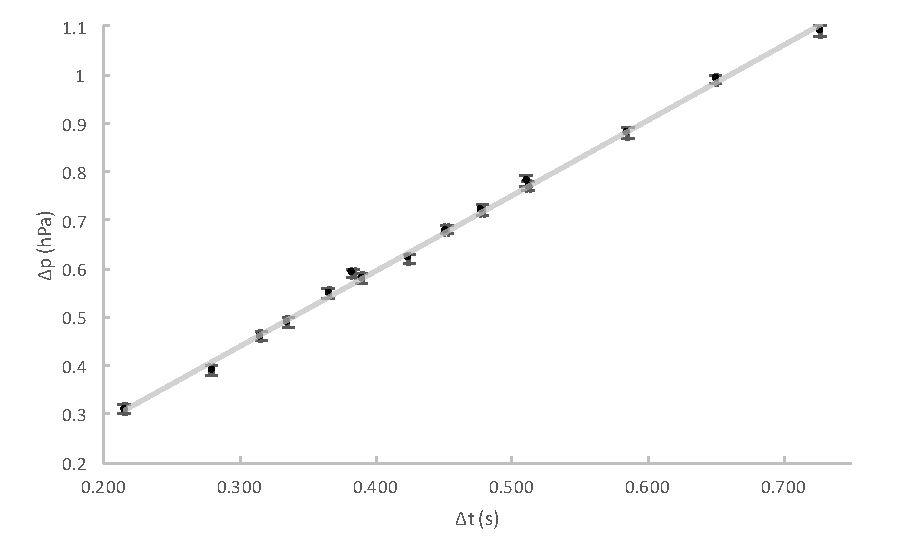
\includegraphics[width=8cm]{fig1}
\caption[]{The maximum rise in pressure recorded as a function of heating time. The error bars on the time are too small to be seen.}
\label{fig:fig1}
\end{center}
\end{figure}


\vspace{-3ex}
\section{Equation, maths, and symbols} 
\vspace{-2ex}

The experiment considered here is an attempt at measuring C\textsubscript{V} for air at room temperature and at atmospheric pressure. Air can be considered to be an ideal gas in the present context. If the volume of air is heated up,\textit{V}, is constant, the change in pressure $\Delta p$ produced by a change in temperature $\Delta T$ can therefore be obtained from the ideal-gas law, $\Delta pV = \textit{nR$\Delta T$} $ , where \textit{R} is the gas constant. Hence, 


\begin{equation} \tag{2}
C\textsubscript{V} = \frac{QR}{\Delta pV}\\
\end{equation}


 
\vspace{-3ex}
\begin{acknowledgements}
\vspace{-3ex}
The author would like to thank Google with all it's help with LateX, and also TexShop for not breaking on me, and also coffee for allowing me to pull through this long long evening.
\end{acknowledgements}




\end{document}